\documentclass{article}
\usepackage[utf8]{inputenc}
\usepackage{amsmath}
\usepackage{amsfonts}
\usepackage{amssymb}
\usepackage{geometry}
\geometry{margin=1in}
\usepackage{microtype}
\usepackage{graphicx}
\usepackage{subcaption}
\usepackage{float}

\title{July 2025 Summary}
\author{Research Notes}
\date{July 2025}

\begin{document}
\maketitle

\section{July 2025 Research Summary}

\subsection{Galene-Simulator Comparison for 2D Nanowire Structures}
Comprehensive comparison between Galene and our simulator for 2D nanowire structures.

First, I expanded the current Galene code in our simulator. It is now a comprehensive Galene converter which can convert Galene simulation results (.OSV files and .GEO files) into other formats as required, such as MATLAB or for TikZ plots.

For comparison, I present the electron density and potential at a surface plot and at a slice here. The device structure we simulated is a double gate MOS structure, serving as the starting point to study the nanowire MOSFET. Here we use voltages for both gates $V_{gt}$ and $V_{gb}$ of 1.0 V and also a drain voltage $V_d$ of 1.0 V, with velocity saturation neglected (the saturation velocity in Galene is set to $10^{20}$ cm/s while velocity saturation in our simulator is turned off).

\begin{figure}[htbp]
    \centering
    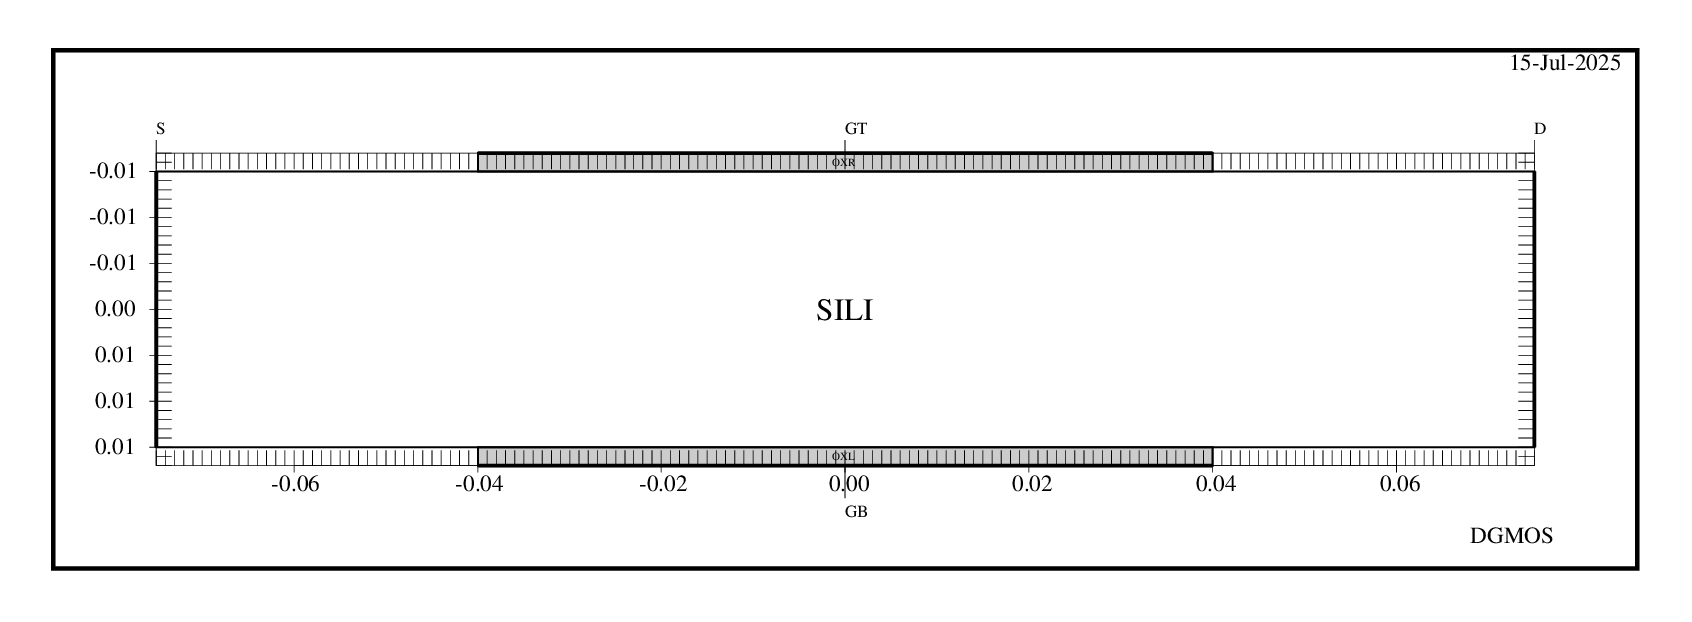
\includegraphics[width=0.8\textwidth]{Figs/dgmos.png}
    \caption{Double gate MOS device structure used as the foundation for nanowire MOSFET studies. Device parameters: length $L = 150$ nm, width = 30 nm, gate length $L_g = 80$ nm, doping regions $L_{dop} = 35$ nm, with doping concentrations $N_{d1} = 10^{20}$ cm$^{-3}$ and $N_{d2} = 10^{15}$ cm$^{-3}$. Oxide thickness $d_{ox} = 2$ nm.}
    \label{fig:dgmos}
\end{figure}

\begin{figure}[H]
    \centering
    \begin{subfigure}[b]{0.48\textwidth}
        \centering
        \includegraphics[width=\textwidth]{Figs/pot_comp.pdf}
        \caption{Potential density comparison}
        \label{fig:potential_comp}
    \end{subfigure}
    \hfill
    \begin{subfigure}[b]{0.48\textwidth}
        \centering
        \includegraphics[width=\textwidth]{Figs/ndens_comp.pdf}
        \caption{Electron density comparison}
        \label{fig:ndens_comp}
    \end{subfigure}
    \caption{Comparison between Galene and our simulator for the 2D nanowire structure. For both subfigures: the first row shows the simulation result from Galene, the second row shows the result from our simulator, the third row is the difference between the two.}
    \label{fig:comparison}
\end{figure}

From the simulation results, it can be seen that the potential and electron density are in good agreement between Galene and our simulator. For the potential difference, it is mainly due to how the simulator handles the region outside the solution domain. As for the carrier density, the deviation is mainly at the doping transition region, which is expected due to different doping mapping approaches used by both simulators.

Here, a comparison of the potential and electron density at a cross-sectional slice is shown. This represents the profile along the surface at y=0.

\begin{figure}[H]
    \centering
    \begin{subfigure}[b]{0.48\textwidth}
        \centering
        \includegraphics[width=\textwidth]{Figs/pot_x_cut.pdf}
        \caption{Potential density slice comparison}
        \label{fig:potential_slice}
    \end{subfigure}
    \hfill
    \begin{subfigure}[b]{0.48\textwidth}
        \centering
        \includegraphics[width=\textwidth]{Figs/ndens_x_cut.pdf}
        \caption{Electron density slice comparison}
        \label{fig:ndens_slice}
    \end{subfigure}
    \caption{Cross-sectional comparison between Galene and our simulator along the y=0 surface.}
    \label{fig:slice_comparison}
\end{figure}


Up to this point, the grid spacing is set to 1 nm for both simulators. Figure~\ref{fig:refined_comparison} shows that after using a refined grid (0.5 nm) in Galene, the deviation regarding the electron density is reduced.
\textbf{Note:} The doping profile mapping into Galene is still under investigation. Our simulator uses a node (vertex) centered doping mapping, while it remains to be confirmed whether Galene uses the same approach or an element-centered mapping.

\begin{figure}[H]
    \centering
    \begin{subfigure}[b]{0.48\textwidth}
        \centering
        \includegraphics[width=\textwidth]{Figs/ndens_zoom_comp.pdf}
        \caption{Electron density comparison at slice with 1 nm and 0.5 nm grid spacing}
        \label{fig:ndens_zoom}
    \end{subfigure}
    \hfill
    \begin{subfigure}[b]{0.48\textwidth}
        \centering
        \includegraphics[width=\textwidth]{Figs/ndens_comp_refined.pdf}
        \caption{Refined grid electron density comparison}
        \label{fig:ndens_refined}
    \end{subfigure}
    \caption{Grid refinement analysis showing electron density comparison. (a) Comparison at a slice with grid spacing of 1 nm and 0.5 nm. (b) Demonstrates that with a refined grid, the deviation between simulators is reduced.}
    \label{fig:refined_comparison}
\end{figure}

\subsection{Vertical FET Structure with Perforated Source}

\subsubsection{VOFET (Vertical Organic Field-Effect Transistor)}

\paragraph{Device Architecture}
Vertical field-effect transistors (VFETs) stack source and drain vertically so the channel length is set by the semiconductor thickness, enabling high current density even in low-mobility materials. A key "pure" VFET variant replaces the compact source with a patterned (perforated) source electrode placed between gate/dielectric and the semiconductor. This geometry mitigates electrostatic screening by the source, avoiding the need for super-capacitive (ion-based) dielectrics and lowering the frequency penalty typical of electric-double-layer gates. In practice, patterned sources can be realized as metal grids (e.g., via block-copolymer lithography) or conductive porous networks (e.g., CNT films), with channel length $L$ defined by the active-layer thickness and device area by the overlap of gate/source/drain.

\paragraph{Operating Principle}
In unbiased devices, both source and drain are blocking (Schottky-like) contacts, so current is contact-limited (CL) and well described by field-enhanced thermionic emission. Under gate bias, the electric field concentrates on the perforation sidewalls (the patterned-electrode/semiconductor interface inside the holes), reducing the injection barrier locally. Charge then accumulates at the perforation bottoms and behaves as an ohmic reservoir (\textbf{"virtual contact"}), shifting the device into a space-charge-limited (SCL) regime where current is controlled by bulk transport rather than injection. Moreover, the spatial origin of ON and OFF currents is different (perforation sidewalls vs. the source top facet), which explains the distinct ON/OFF behaviors.

\paragraph{Complementary Gate Control Modes}
Two complementary gate actions control current:
\begin{enumerate}
    \item \textbf{Virtual contact formation (normally-OFF $\rightarrow$ ON):}
    Gate bias focuses lateral fields on the perforation sidewalls of the source, lowers the Schottky barrier there, and extracts carriers into the perforation bottom. This accumulated charge acts like an ohmic "virtual contact", launching a vertical space-charge channel toward the drain. ON current is then mobility-/space-charge-limited rather than contact-limited.
    
    \item \textbf{Gate-induced internal barrier (normally-ON $\rightarrow$ OFF):}
    With opposite gate polarity (for n-type, negative $V_G$), the gate creates a laterally oriented potential ridge between the patterned source and the drain that repels already injected carriers—analogous to a solid-state triode grid—so the device turns off. The barrier height grows roughly linearly with $|V_G|$ and decays exponentially away from the perforation edge.
\end{enumerate}

A practical consequence of the geometry is an "inversion point" above each perforation: along the perforation axis the vertical field flips sign; the potential difference from the perforation bottom to this point behaves like an effective barrier that controls how much charge reaches the upper channel. Moving this inversion point upward (e.g., with thicker $h_s$) degrades ON current and ON/OFF ratio.

\paragraph{Limiting Current Regimes}
The patterned-electrode VFET admits two robust limiting forms that are convenient for analysis and parameter extraction:

\begin{itemize}
    \item \textbf{OFF (CL) regime} — injection from the source top facet:
    \begin{equation}
    J_{\mathrm{OFF}} = q \ln N_0 E_\perp \exp\left(-\frac{q u_b}{kT}\right) (1-\text{FF})
    \end{equation}
    with image-force barrier lowering $u_b = u_{b0}-\sqrt{qE_\perp/(4\pi\varepsilon_0\varepsilon)}$ and $E_\perp \approx V_{DS}/L_{\mathrm{OFF}}$. The factor $(1-\text{FF})$ accounts for conduction only through the non-perforated area.
    
    \item \textbf{ON (SCL) regime} — injection from perforation sidewalls (virtual contact):
    \begin{equation}
    J_{\mathrm{ON}} = \frac{9}{8} \varepsilon_0\varepsilon \mu \frac{V_{DS}^2}{L^{3}} \text{FF}
    \end{equation}
    reflecting that ON current originates from the perforation area.
\end{itemize}

Dividing the SCL by the CL form gives a compact expression for the ON/OFF ratio that highlights the roles of fill factor FF, channel length $L$, and especially the intrinsic barrier $\phi_{b0}$ at the patterned-electrode/semiconductor interface (the analysis is most accurate when $\phi_{b0} \gtrsim 0.7$ eV so the CL description is valid).

\paragraph{Geometry-Performance Relationships}
Two geometric levers dominate:
\begin{itemize}
    \item \textbf{Source thickness $h_s$ ("tunnel"/shielding effect):} Increasing $h_s$ raises the aspect ratio (thickness/diameter), which confines the virtual contact within the perforation and shields it from the drain field, reducing ON current and ON/OFF ratio (experimentally, a $\sim$5× drop moving from $h_s \sim 7$ nm to 13 nm was observed). Edge morphology matters: spiky edges enhance confinement; smoother edges help.
    
    \item \textbf{Perforation diameter $D$, fill factor FF, and dielectric thickness $h_d$:} Larger FF boosts ON current (more active sidewall length) while reducing the OFF conduction area. Electrostatics scale with the $h_d$:$D$ ratio (well-behaved devices favor $h_d$:$D \gtrsim 1$:3); increasing $D$ has a similar effect to decreasing $h_d$.
\end{itemize}

These observations rationalize why thin, highly perforated sources with well-controlled sidewalls maximize ON current without compromising OFF suppression.

\paragraph{Boundary Conditions}
State-of-the-art analyses solve 2D Poisson + steady-state drift–diffusion with Scharfetter–Gummel discretization. The electrostatic potential is solved everywhere (metals, dielectric, semiconductor), while carrier densities are solved only inside the semiconductor; thus, some BCs are interior (at metal/semiconductor and dielectric/semiconductor interfaces). Metals are treated with negligible Debye length (fixed work functions). Electrode BCs for potential are Dirichlet with applied biases ($V_G$, $V_S = 0$, $V_D$) plus a contact potential $u_{b0}$. 

Carrier BCs at metal/semiconductor assume local thermionic equilibrium with field-lowered barrier:
\begin{equation}
n = N_0 \exp\left(-\frac{q u_b}{kT}\right), \quad u_b = u_{b0}-\Delta u \approx u_{b0}-\Delta x E_\perp
\end{equation}
with $\Delta x$ taken as an intermolecular/mesh scale ($\sim$1 nm). Lateral BCs are cyclic/periodic at the unit-cell sidewalls to represent an infinite perforation array. At the dielectric/semiconductor interface at each perforation bottom, the interface is treated as insulating (no surface charge, zero normal current). Numerically, charge-neutral initial conditions and damped iterations are used for robust convergence.

\paragraph{Implications for Perovskite VFETs}
Perovskites introduce mixed ionic–electronic transport and defect-rich energetics. In practice, retain the electronic BCs above, but extend the model to include ionic continuity equations with blocking or partially blocking ionic BCs at metals and dielectrics (to capture gate-field screening, hysteresis, and time-dependent turn-on). Where OFF leakage via the source top facet is significant, include image-force barrier lowering in CL fits (analytical term as above) and consider field-dependent mobility and trap-assisted recombination within the semiconductor.

\subsubsection{Current Simulation Approach}

Since we do not have Schottky contacts implemented in our simulator, the current workaround is to use a partially doped active layer with ohmic contacts as a substitute for the Schottky contact. This approach allows us to proceed with simulations while we work on integrating the Schottky contact feature into our simulator.

The structure used is a partial element which contains the gate at the bottom, the dielectric layer above, a section of the perforated source alongside the gap between the sources, the active layer above, and the drain contact with the following parameters:

\begin{verbatim}
# Vertical FET dimensions
L_total = 200        # Total device width (nm)
x0 = -100           # Left boundary
xL = 100            # Right boundary
x_s = 0             # Source/aperture boundary (creates 100nm source + 100nm aperture)

d_ox = 5            # Gate oxide thickness (nm)
y_ox = 5            # Top of gate oxide
y_s = 25            # Top of source layer (20nm source thickness)
y_d = 55            # Top of active layer (30nm channel length)

# Doping levels
Nd_light = 1e15    # Light doping for channel
Nd_heavy = 1e20    # Heavy doping for aperture
\end{verbatim}

The schematic is shown in the figure below.

\begin{figure}[H]
    \centering
    % placeholder for figure
    \caption{Schematic of the VFET structure with partial doping}
    \label{fig:vfet_schematic}
\end{figure}

With the gate voltage $V_g$ set to 0.1 V (which should be irrelevant in this case since the original purpose of the gate voltage is to form the carrier reservoir or virtual contact, and with our setup this is already formed) and a drain voltage of 1 V, we have the following results:

\begin{figure}[H]
    \centering
    % placeholder for figure  
    \caption{Simulation results for the VFET structure}
    \label{fig:vfet_results}
\end{figure}

Eventually, we will need to implement the correct physics to show the proper current direction and other characteristics.


\subsection{Schottky Contact Implementation}
The current version of our simulator does not support Schottky contacts. To simulate devices like RFETs or VFETs, the implementation of Schottky contacts is necessary.

For the current ohmic contact, we have charge neutrality $n_0-p_0 = N_D - N_A$ and assume equilibrium, which for Boltzmann statistics gives:
\begin{equation}
\phi = V_k + \frac{kT}{q} \text{asinh} \left( \frac{N_D - N_A}{2 n^2_{i,\text{eff}}} \right)
\end{equation}

In the Schottky contact case, the following expression is used:
\begin{equation}
\phi = V_k - \phi_B + \frac{kT}{q} \ln \left( \frac{N_C}{n_{i,\text{eff}}} \right)
\end{equation}

Another aspect to consider is the different type of boundary condition. Instead of the Dirichlet BC, a Robin (mixed) BC is used, which gives:
\begin{equation}
\vec{J}_n \cdot \vec{n} = q v_n (n-n^B_0)
\end{equation}
\begin{equation}
\vec{J}_p \cdot \vec{n} = q v_p (p-p^B_0)
\end{equation}
with
\begin{equation}
n^B_0 = N_C \exp\left(-\frac{q\phi_B}{kT}\right)
\end{equation}
and 
\begin{equation}
p^B_0 = N_V \exp\left(-\frac{q(\chi + E_g - \phi_B)}{kT}\right)
\end{equation}

where $\phi_B$ is the barrier height (the difference between the contact work function and the electron affinity of the semiconductor). $v_n$ and $v_p$ are the thermoionic emission velocities for electrons and holes, respectively. $n^B_0$ and $p^B_0$ are the equilibrium densities at the Schottky contact.



\subsection{Next Steps}
\begin{itemize}
    \item Complete pending comparison plots
    \item Analyze results from refined grid simulations
    \item Document discrepancies and alignment patterns between simulators
    \item Prepare formal write-up for main paper draft
\end{itemize}

\end{document}
